In this section, we introduce the architecture used for deep CNN. We obtain an efficient feature extractor by fine-tuning the GoogLeNet incorporating the data from ImageNet. We achieve the-state-of-the-art performance on Food-101 dataset and show that with deep representation and just a few examples from each food category in Food-101, linear model can achieve competitive result compared to model trained on full dataset on Food-101. We also discuss some features we find for GoogLeNet in comparison with AlexNet \cite{krizhevsky2012imagenet} in this section to see the advantage of GoogLeNet.
\subsection{Architecture of GoogLeNet}
The architecture of deep CNN would greatly affects the performance of the feature extractor and optimized architecture leads to efficient feature representation.
Instead of exploring our own deep CNN architecture, we decide to use the existing one, GoogLeNet. GoogLeNet achieved 93.33\% top-5 accuracy on a 1000-category image recognition task which is very close to the performance of human annotation \cite{szegedy2014going}. We believe that its architecture can help us extract efficient deep feature representations for our adaptation task.

 The architecture of GoogLeNet is unique to other deep CNN. Inspired by \cite{linNiN}, small $1\times 1$ receptive field are intensively used throughout the network. There are 9 "Inception" modules in GoogLeNet and Figure \ref{incept} shows the architecture of a single inception module. Another interesting feature of GoogLeNet is that there are two extra auxiliary classifiers in intermediate layers. During the training procedure, the loss of these two classifiers are counted into the total loss with a discount weight 0.3, in addition with the loss of the classifier on top. More details of its architecture can be found from \cite{szegedy2014going}.

\begin{figure}
  \centering
  % Requires \usepackage{graphicx}
  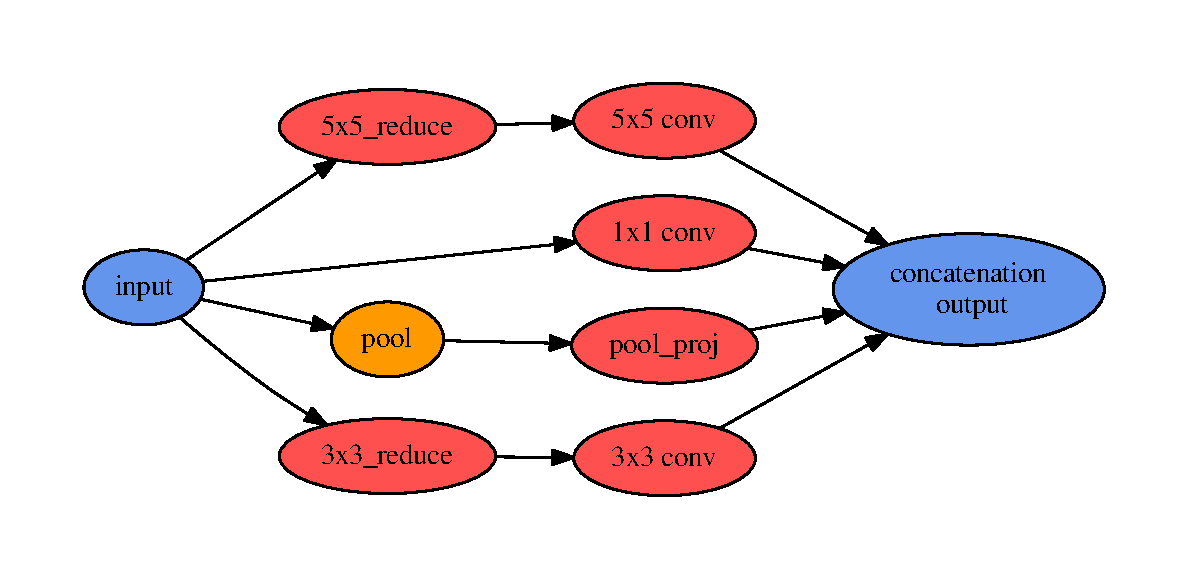
\includegraphics[scale=.45]{fig/inception.pdf}\\
  \caption{Inception Module. $n\times n$ stands for size $n$ receptive field, $n\times n\_reduce$ stands for the $1\times 1$ convolutional layer before the $n\times n$ convolution layer and $pool\_proj$ is another $1\times 1$ convolutional layer after the MAX pooling layer. The output layer concatenates all its input layers.}\label{incept}
\end{figure}

\subsection{Pre-training and Fine-tuning GoogLeNet}
Indeed, even training a deep CNN directly with over a million labeled examples should be very careful to prevent overfitting \cite{krizhevsky2012imagenet}.
Because the training set of Food-101 contains only 75,750 images, training GoogLeNet on it directly can be easily prone to overfitting. But the idea of supervised pre-training on some huge image datasets could preventing this problem in certain degree. Compared to other randomly initialized strategies with certain distribution, supervised pre-training is to initialize the weights according to the model trained from another specific task. Initialization with pre-trained model has certain bias as there is no single dataset including all the invariance for natural images , but the bias can be reduced as the size of the pre-trained image dataset increases \cite{agrawal2014analyzing}. So the fine-tuning the model on small dataset should benefit from it.

To compare the result of GoogLeNet with other deep CNN model, we use the AlexNet as the baseline of deep CNN.
We conduct several experiments on both architectures and use different training initialization strategies for Food-101 datasets. In our experiment, the scratch models are initialized with Gaussian distribution for AlexNet and Xavier algorithm for GoogLeNet \cite{glorot2010understanding}. These two initialization strategies are used for training the original models for the ImageNet task. The ft-last and fine-tuned models are initialized with the weights pre-trained from ImageNet dataset. But for the ft-last model, we just re-train the fully connected layers while the whole network is fine-tuned for the fine-tune model.
% Table generated by Excel2LaTeX from sheet 'Sheet1'
\begin{table}[htbp]
  \centering
  \caption{Top-5 Accuracy for different deep cnn architectures}
    \begin{tabular}{r|ccc}
    \toprule
          & Fine-tune & Ft-last & Scratch \\
    \midrule
    GoogLeNet & \textbf{93.51} & 82.84 & 90.45 \\
    AlexNet & \textbf{88.12} & 78.18 & 76.49 \\
    \bottomrule
    \end{tabular}%
  \label{tab:ft}%
\end{table}%



% Table generated by Excel2LaTeX from sheet 'Sheet1'
\begin{table*}[htbp]
  \centering
  \caption{Top-1 accuracy compared to other methods on Food-101 dataset in percent}
    \begin{tabular}{c|C{3cm}C{3cm}cc}
    \toprule
          & RFDC\cite{bossard2014food} & MLDS($\approx$\cite{singh2012unsupervised}) & GoogLeNet & AlexNet \\
    \midrule
    Top1 accuracy & 50.76 & 42.63& \textbf{78.11 }& 66.40 \\
    \bottomrule
    \end{tabular}%
    \label{tab:101}
\end{table*}%
% Table generated by Excel2LaTeX from sheet 'Sheet1'
\begin{table*}[htbp]
  \centering
  \caption{Accuracy for different number of examples in each category}
    \begin{tabular}{c|c|c|c|c|c|c}
    \toprule
        &\multicolumn{6}{c}{Number of examples in each category }\\
        \midrule
          & Full (750)   &  5     & 4     & 3     & 2     & 1 \\
    \midrule
    Top-1  & 78.11& 72.53 $\pm$ 0.36& 71.07 $\pm$ 0.49& 69.11 $\pm$ 0.84& 64.94 $\pm$ 0.93& 63.62 $\pm$ 1.79 \\
    Top-5  & 93.51 & 90.35 $\pm$ 0.26& 89.56 $\pm$ 0.31 & 88.41 $\pm$ 0.48   & 86.14 $\pm$ 0.52& 79.05 $\pm$ 1.37 \\
    \bottomrule
    \end{tabular}%
  \label{tab:mini}%
\end{table*}%


\begin{figure*}[htbp]
  \centering
  % Requires \usepackage{graphicx}
  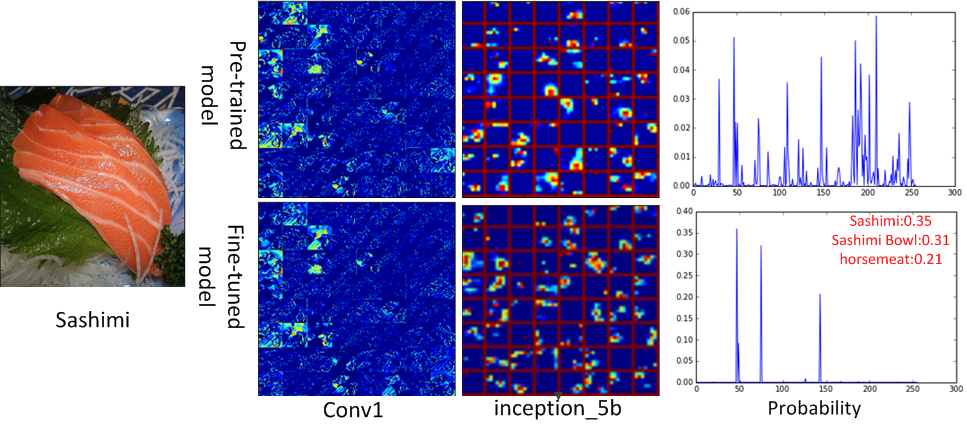
\includegraphics[scale=0.5]{fig/sashimi.png}\\
  \caption{Visualization of some feature maps of GoogLeNet models in different layers for the same input image. 64 feature maps of each layer are shown. Conv1 is the first convolutional layer and Inception\_5b is the last convolutional layer. }
   \label{fig:sashimi}
\end{figure*}
From Table \ref{tab:ft} we can see that fine-tuning the whole network can improve the performance of the CNN for our task. Compared to other shallow models (see Table \ref{tab:101}), GoogLeNet outperforms the other methods with large margins and we provide the state-of-the-art performance on this dataset.

In \cite{farabet2013learning}, Deep CNN is proved to learn hierarchical hierarchical feature representations automatically.
In Figure \ref{fig:sashimi} we visualize the feature maps of the pre-trained GoogLeNet model and fined-tuned GoogLeNet model with the same input image for some layers. We can see that the feature maps of the lower layer are similar as the lower level features (such as features for lines and edges detection etc.) are similar for most recognition tasks.
Then we can see that the feature maps in the high-level are different which leads to totally different recognition results.
Since only the last layer (auxiliary classifier) of the ft-last model is optimized, we can infer that the higher level features are more important which is consistent with our intuition. %Also from Table \ref{tab:ft}, it is interesting to see that even though Food-101 is a relative large dataset with 750 training examples per category, the model can still takes advantage of the initialization from ImageNet dataset.

From previous work, deep feature representation from CNN has shown some impressive results for fine-grained recognition, which suggests that deep feature representation can learn distinctive features from similar categories \cite{zhang2014part} \cite{razavian2014cnn}. We shows the weight similarity of the linear auxiliary classifier and average representation similarity in GoogLeNet for some similar foods in Food-101 dataset in Table \ref{tab:weight_sim} and \ref{tab:pre_sim}. We can observe that the different representation eventually leads to different weights of the linear classifier.
Moreover, we find that with deep representation from GoogLeNet, we can achieve similar accuracy while just using a few labeled examples from each category.
We use deep representation from GoogLeNet as the input of logistic regression classifier and compare the results of different number of training examples on Food-101 dataset.
Table \ref{tab:mini} shows the average accuracy of the models on different number of examples in each category compared with model trained on full dataset. We can see that even though size of the training examples is significantly reduced, the performance of the classifier is not greatly degraded.
This suggests that GoogLeNet can learn fine-grained feature representations on Food-101 which could be efficient way to alleviate the dataset bias for adaptation. In Section \ref{sec:da}, we use the deep feature representation extracted from fine-tuned GoogLeNet as the input for our incremental domain adaptation method.
% Table generated by Excel2LaTeX from sheet 'Sheet1'
\begin{table}[htbp]
  \centering
  \caption{Cosine similarity of the weights for similar foods}
    \begin{tabular}{c|c|c}
    \toprule
          & Caprese salad & Greek salad \\
    Caesar salad & 0.1406 & 0.3155 \\
    \toprule
          & Carrot cake & Cup cakes \\
    Cheesecake & 0.1711 & 0.1276 \\
    \toprule
          & Grilled cheese sandwich & Hamburger \\
    Club sandwich & 0.2866 & 0.2303 \\
    \bottomrule
    \end{tabular}%
  \label{tab:weight_sim}%
\end{table}%
\begin{table}[htbp]
  \centering
  \caption{Average cosine similarity of the representation for similar foods}
    \begin{tabular}{c|c|c}
    \toprule
          & Caprese salad & Greek salad \\
    Caesar salad & 0.4005& 0.5612 \\
    \toprule
          & Carrot cake & Cup cakes \\
    Cheesecake & 0.4952 & 0.4561 \\
    \toprule
          & Grilled cheese sandwich & Hamburger \\
    Club sandwich & 0.6651 & 0.6038 \\
    \bottomrule
    \end{tabular}%
  \label{tab:pre_sim}%
\end{table}%

\subsection{Advantage of GoogLeNet for fine-tuning}
In the last part, we obtain an efficient feature extractor on Food-101 dataset with the architecture of GoogLeNet. In this part, we introduce some of our findings that makes GoogLeNet efficient.

Training a neural network is essentially adjusting the parameters of the network to minimize the empirical risk. Different from any previous architectures \cite{krizhevsky2012imagenet} \cite{simonyan2014very}, the GoogLeNet consists of several stacked Inception modules. We find that GoogLeNet model can learn the kernel weights of each layer more efficiently while the model with other architecture (we take AlexNet for contrast in this paper) would suffer from vanished gradient a lot.

From Table \ref{tab:ft} we can see that GoogLeNet outperforms AlexNet which implies that the deep feature representations of GoogLeNet are more distinctive compared to AlexNet.
To illustrate the changes of the weights for different architectures after fine-tuning, we calculate the weights' cosine similarity of each layer between the fine-tuned models and their pre-trained models and show them in table \ref{tab:cosg} and \ref{tab:cosa}. Because the pre-trained models are used for general recognition task, for our specific food recognition task, we expect a model that can learn features only for food recognition. Therefore, the weights of the model should be greatly adjusted to better fit our new scenario.

From Table \ref{tab:cosa}, we can observe that the weights of the pre-trained and fine-tuned models are extremely similar in AlexNet which we believe is caused by vanished gradient.
Vanished gradient is a difficulty for deep neural network while errors propagate shrink greatly as it goes deeper \cite{glorot2010understanding}. This makes the network difficult to fit the data and degrades its performance. Even though ReLUs is proposed to alleviate this problem in \cite{NairH10} and used in both architectures,
from Table \ref{tab:cosg} and \ref{tab:cosa} we can see that they still suffer from this problem. However, GoogLeNet suffers significantly less. This indicates that GoogLeNet could be more flexible to fit the new examples which is consistent with the results in Table \ref{tab:ft}.

By comparing the changes of weights in fine-tuning, we can see that training GoogLeNet is more easy and achieve better result.
%We find that Inception module in GoogLeNet can make the network learn better features.

%Rectified activation function is mathematically given by:
%      \begin{equation}\label{relu}
%        h = \max ({w^T}x+b,0) = \left\{ {\begin{array}{*{20}{c}}
%{{w^T}x+b}&{{w^T}x+b > 0}\\
%0&{else}
%\end{array}} \right.
%      \end{equation}
%
%    The ReLU is inactivated when its input is below 0 and its partial derivative is 0 as well. ReLU can naturally generate sparse representation as well as sparse back propagation error.
%    The derivative of the filter for backpropagetion is $\frac{{\partial J}}{{\partial w}} = \frac{{\partial J}}{{\partial y}}\frac{{\partial y}}{{\partial w}} = \frac{{\partial J}}{{\partial y}}*x$ where $\frac{{\partial J}}{{\partial y}}$ denotes the partial derivative of the activation function, $y=w^Tx+b$ and $x$ denotes the inputs of the layer. ReLUs can generate sparse feature representation and improve the performance of the linear classifier for image classification \cite{lee2006efficient}. But on the other hand, for each layer, sparser input is more likely to make the net more difficult to train. The sparse input and ReLUs could lead to sparse filter derivative which would more likely to keep the weights unchanged. Therefore, fine-tuned AlexNet model is extremely similar to the pre-trained one. Compared to large receptive field used in AlexNet, the inception module in GoogLeNet contains 2 additional $n\times n\_reduced$ convolutional layers before the $3\times 3$ and $5\times 5$ convolutional layers (see Figure \ref{incept}). We calculate the Sparsity of the output for each unit in GoogLeNet inception module on training set of Food-101 in Table \ref{tab:sparse}. From Table \ref{tab:sparse} we can see that the outputs of the  $n\times n\_reduced$ units are denser than  $n\times n$ units. Even though the original purpose of these two $1\times 1$ convolutional layer is for computational efficiency \cite{szegedy2014going}, these 2 convolutional layers tend to squeeze their sparse inputs and generate a dense outputs for the following layer. We calculate the sparsity of each unit in GoogLeNet inception module for training data from Food101 in Table \ref{tab:sparse}. We can see from Table \ref{tab:sparse} that the sparsity of the $n\times n\_reduce$ layers are denser than other layers within the inception module. This makes the filters in the following layer more easily to be trained for transfer learning and generate efficient sparse representations.


\begin{table*}[htbp]
  \centering
  \caption{Cosine similarity of the layers in inception modules between fine-tuned models and pre-trained model for GoogLeNet}
    \begin{tabular}{r|cccccc}
    \toprule
    \multicolumn{7}{c}{food101} \\ \midrule
          & \multicolumn{1}{l}{1x1 } & \multicolumn{1}{l}{3x3\_reduce} & \multicolumn{1}{l}{3x3} & \multicolumn{1}{l}{5x5\_reduce} & \multicolumn{1}{l}{5x5} & \multicolumn{1}{l}{pool\_proj } \\
    inception\_3a & 0.71  & 0.72  & 0.63  & 0.67  & 0.73  & 0.68 \\
    inception\_3b & 0.56  & 0.63  & 0.50  & 0.71  & 0.60  & 0.53 \\
    inception\_4a & 0.43  & 0.50  & 0.50  & 0.47  & 0.62  & 0.36 \\
    inception\_4b & 0.48  & 0.52  & 0.57  & 0.50  & 0.67  & 0.35 \\
    inception\_4c & 0.57  & 0.61  & 0.59  & 0.53  & 0.63  & 0.47 \\
    inception\_4d & 0.54  & 0.58  & 0.53  & 0.54  & 0.64  & 0.44 \\
    inception\_4e & 0.53  & 0.54  & 0.61  & 0.55  & 0.62  & 0.42 \\
    inception\_5a & 0.43  & 0.47  & 0.53  & 0.45  & 0.57  & 0.34 \\
    inception\_5b & 0.36  & 0.39  & 0.46  & 0.38  & 0.52  & 0.37 \\
    \bottomrule
    \end{tabular}%
  \label{tab:cosg}%
\end{table*}%


\begin{table*}[htbp]
  \centering
  \caption{Cosine similarity of the layers between fine-tuned models and pre-trained model for AlexNet}
    \begin{tabular}{r|ccccccc}
    \toprule
          & conv1 & conv2 & conv3 & conv4 & conv5 & fc6   & fc7 \\
    \midrule
    food101 & 0.996 & 0.984 & 0.963 & 0.960 & 0.963 & 0.925 & 0.933 \\
    \bottomrule
    \end{tabular}%
  \label{tab:cosa}%
\end{table*}%

%% Table generated by Excel2LaTeX from sheet 'google'
%\begin{table*}[htbp]
%  \centering
%  \caption{Sparsity of the output for each unit in GoogLeNet inception module for training data from Food101 in percent}
%    \begin{tabular}{r|cccccc}
%    \toprule
%          & 1x1  & 3x3\_reduce & 3x3  & 5x5\_reduce & 5x5  & pool\_proj  \\
%    \midrule
%    inception\_3a & $69.3\pm 1.3$  & $69.6 \pm 1.1$  & $80.0\pm  1.0$& $64.1\pm  2.2$& $75.8\pm  1.6$& $76.2\pm 5.4$\\
%    inception\_3b & $92.8 \pm 0.9$&$ 76.5 \pm 0.9$& $94.7\pm 0.9 $&$ 71.6 \pm 2.3 $&$ 94.4\pm 0.5 $&$ 94.7 \pm 1.6$\\
%    inception\_4a & $90.9 \pm 0.9$& $70.0\pm 1.2 $& $93.8\pm 1.1 $& $63.3\pm 4.0 $& $91.9\pm 1.8 $& $95.1\pm 2.0$\\
%    inception\_4b & $71.9 \pm 1.6$& $67.5\pm 1.2$ & $75.4\pm  1.0$& $58.5 \pm 2.6$& $78.9\pm  1.6$& $85.6\pm 3.6$\\
%    inception\_4c & $75.1 \pm 2.4$& $72.6 \pm 1.3$& $81.0\pm 2.0$ & $66.3\pm 6.1 $& $79.7 \pm 3.6$& $88.1\pm 3.3$\\
%    inception\_4d & $87.3 \pm 2.7$& $78.0 \pm 2.2$& $88.0\pm 1.6$& $67.9\pm 3.1 $& $88.9\pm 2.8 $& $93.0\pm 2.2$\\
%    inception\_4e & $91.8\pm  1.1$& $62.3\pm 2.2 $& $91.0\pm 2.5 $& $49.5 \pm 3.7$& $94.0 \pm 1.0$& $92.3\pm 1.5$\\
%    inception\_5a & $78.7 \pm 1.6$& $66.5\pm  1.7$& $82.3\pm 2.6 $& $59.9\pm 3.2 $& $86.4\pm 2.3 $& $87.1\pm 2.6$\\
%    inception\_5b & $88.2\pm 2.3 $& $86.8 \pm 1.6$&$ 83.3\pm 4.4$ & $84.0\pm 3.1 $& $81.4\pm 5.3$  & $94.7\pm 1.5$\\
%    \bottomrule
%    \end{tabular}%
%  \label{tab:sparse}%
%\end{table*}%

%The unique structure of the Inception module guarantees that the sparse outputs from previous layer can be squeezed within the $1\times 1$ convolutional layers and field to generate sparser representation in the next layer. The squeeze action promises the back propagation error can be transferred more efficiently and makes the whole network more flexible to fit different recognition tasks.

